\chapter{Run conditions and Experimental setup}
\label{chap:physics}

\section{Run Group F conditions}

MH will write this

%%%%%%%%%%%%%%%%%%
\section{The CLAS12 Spectrometer}
%%%%%%%%%%%%%%%%%%
The CLAS12 spectrometer is designed to operate with 11~GeV beam at an 
electron-nucleon luminosity of $\mathcal{L} = 
1\times10^{35}~$cm$^{-2}$s$^{-1}$. The baseline configuration of the CLAS12 
detector consists of the forward detector and the central detector 
packages~\cite{CD} (see Figure~\ref{fig:fd}). We use the forward detector for 
electron and photon detection. The central detector's silicon tracker and 
barrel micromegas will be removed to leave room for the BONuS12 RTPC.  

\begin{figure}
  \begin{center}
    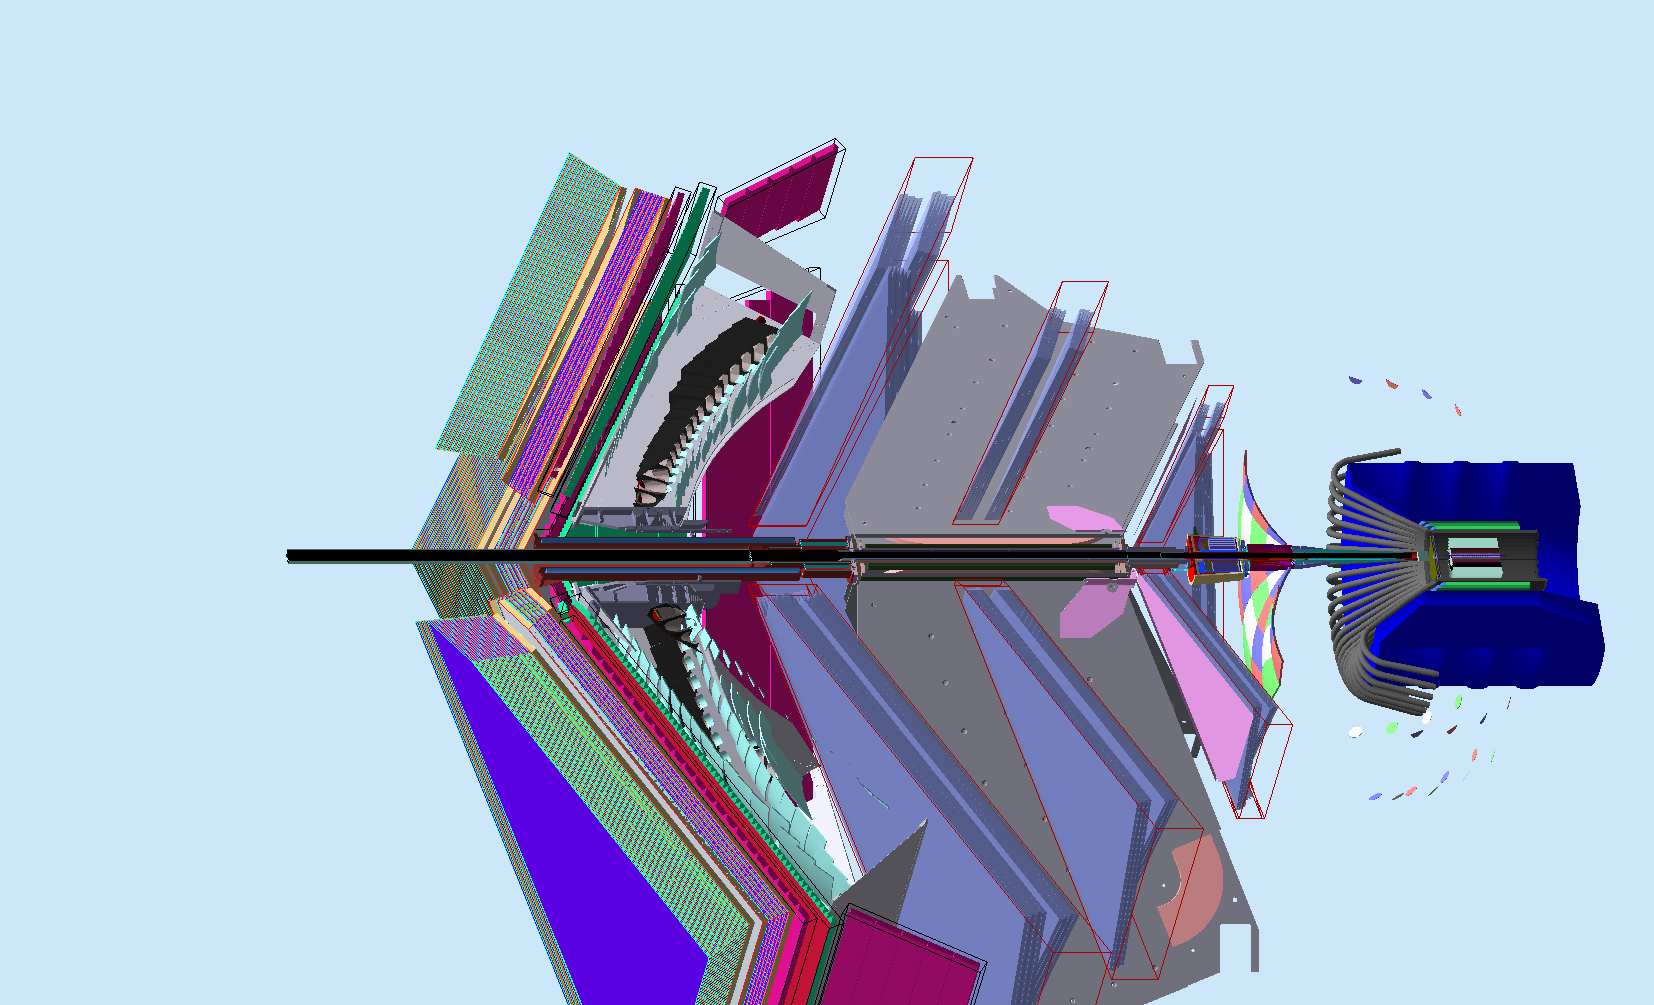
\includegraphics[angle=0, width=0.75\textwidth]{figures/clas12_bonus12.png}
    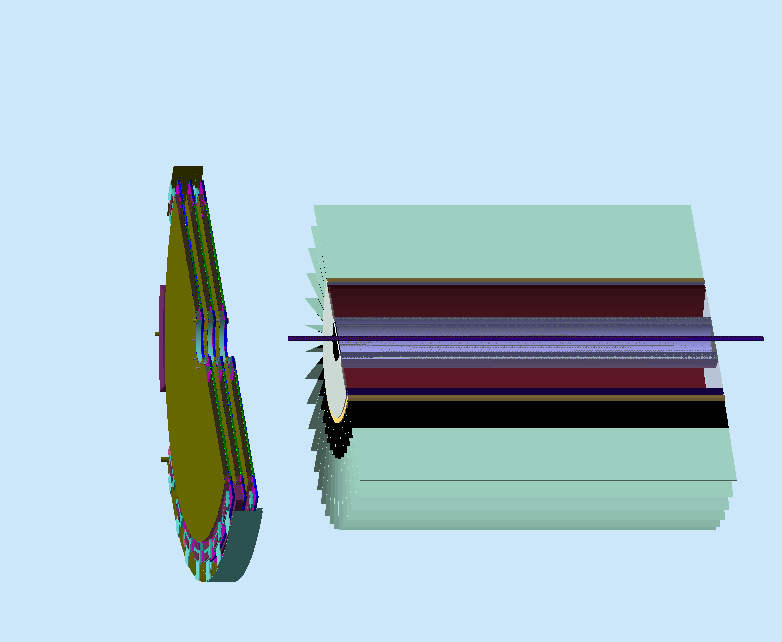
\includegraphics[angle=0, width=0.75\textwidth]{figures/bonus12_fmt.png}
     \caption{(Top) The schematic layout of the CLAS12 baseline design with 
     BONuS12 RTPC replacing the silicon tracker and the barrel micromegas.  
     (Bottom) Schematic layout showing BONuS12 RTPC with the modified design of 
     the forward micromegas.}
    \label{fig:fd}
  \end{center}
\end{figure}

The scattered electrons and photons will be detected in the forward detector which consists 
of the High Threshold Cherenkov Counters (HTCC), Drift Chambers (DC), the Low 
Threshold Cherenkov Counters (LTCC), the Time-of-Flight scintillators (TOF), 
the Forward Calorimeter and the Preshower Calorimeter. The charged particle 
identification in the forward detector is achieved by utilizing the combination 
of the HTCC, LTCC and TOF arrays with the tracking information from the Drift 
Chambers. The HTCC together with the Forward Calorimeter and the Preshower 
Calorimeter will provide a pion rejection factor of more than 2000 up to a 
momentum of 4.9~GeV/c, and a rejection factor of 100 above 4.9 GeV/c. The photons
are detected using the calorimeters.

\section{BONuS12 RTPC} 

\begin{figure}
  \begin{center}
    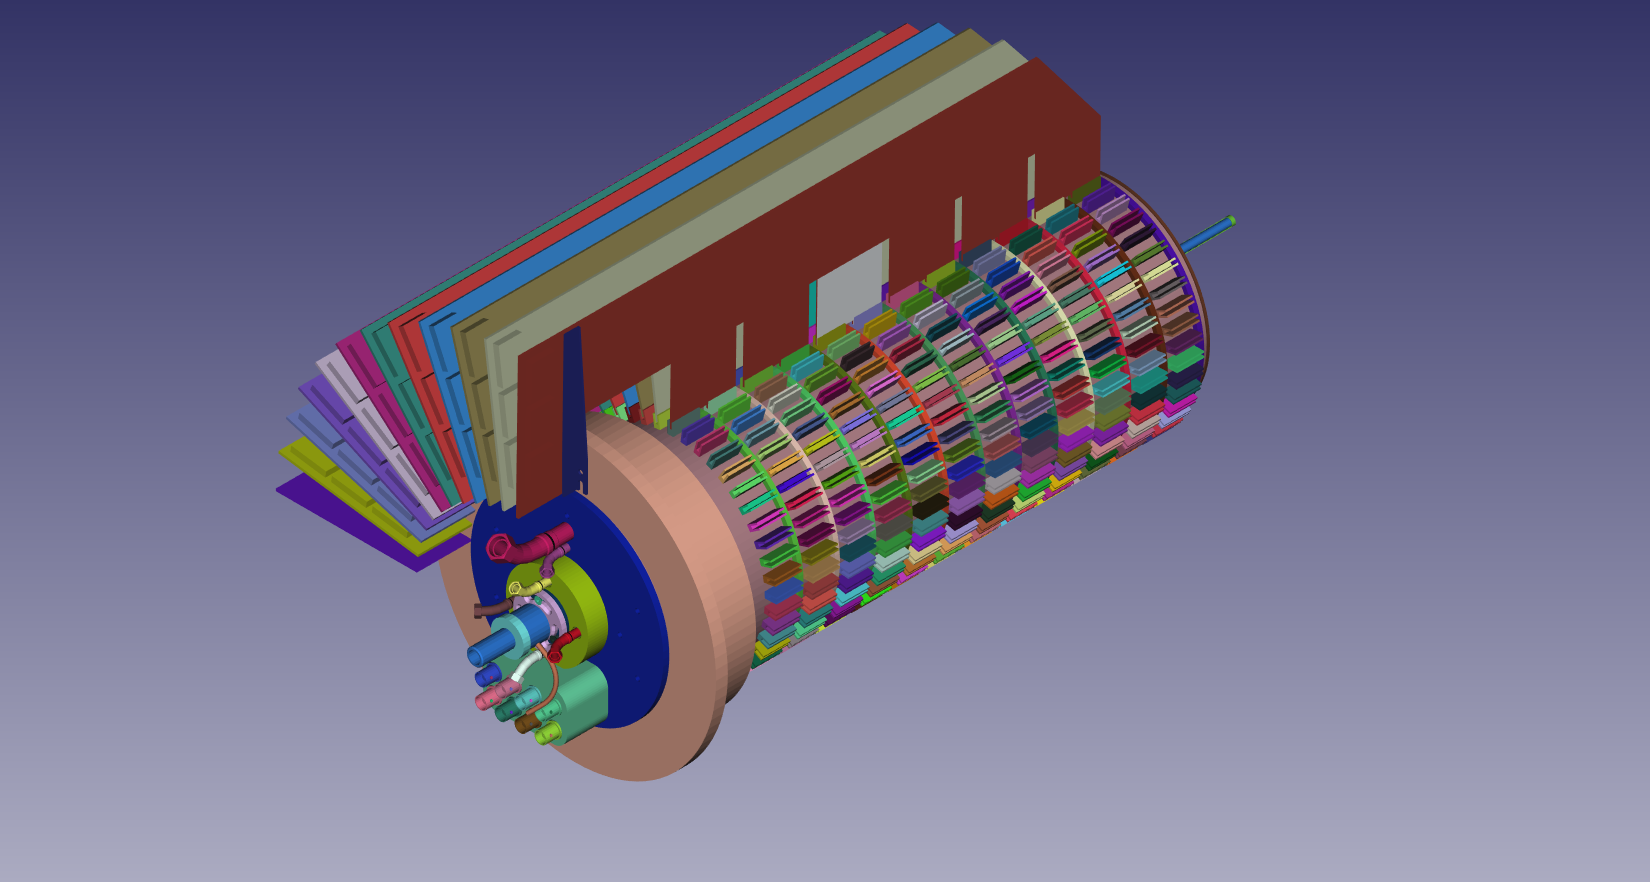
\includegraphics[angle=0, width=0.45\textwidth, clip,trim=50mm 10mm 80mm 
     0mm]{figures/Bonus12_cad.png}
    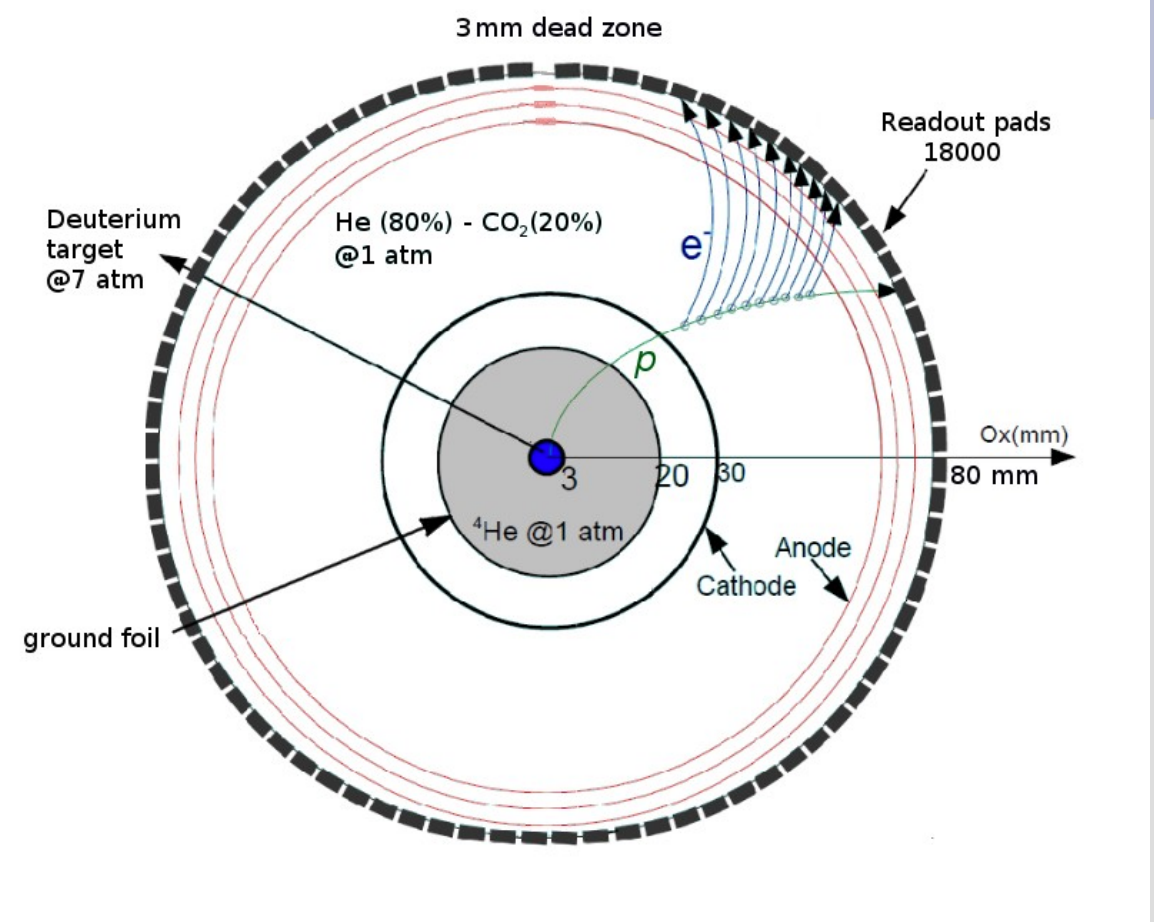
\includegraphics[angle=0, width=0.45\textwidth,clip,trim=0mm 10mm 20mm 0mm 
     ]{figures/NKsBXp.png}
     \caption{(Left) Schematic layout showing BONuS12 RTPC showing the readout 
     padboard and few adaptive boards in addition to the gas lines. (Right) 
     Schematic drawing of the CLAS RTPC in a plane perpendicular to the beam 
     direction. See text for description of the elements.}
    \label{fig:bonus12}
  \end{center}
\end{figure}

The new CLAS12 RTPC (BONuS12) is a active 400~mm long cylinder of 160~mm 
diameter, leaving just enough room to fit adaptive readout boards between the 
RTPC outer shell and the solenoid. The electric field is directed 
perpendicularly to the beam direction, such that drifting electrons are pushed 
away from the beam line. These electrons are amplified by three layers of 
cylindrical gas electron multipliers (GEM)~\cite{Sauli:2016eeu} and detected by 
the readout system on the external shell of the detector as illustrated in 
Figure~\ref{fig:bonus12}.  The RTPC is segmented into two halves with 
independent GEM amplification systems that cover almost 100\% of the azimuthal 
angle range.

RD: Is this Bonus, eg6 or bonus12? Seems like a mix.

We detail here the different regions shown in Figure~\ref{fig:bonus12} starting 
from the beam line towards larger radius:\\
\begin{itemize}
  \item The 7~atm Deuterium gas target extends along the beamline forming the 
     detector central axis. It is a 6~mm diameter Kapton straw with a 50~$\mu$m 
      wall of 492~mm length such that its entrance and exit 15~$\mu$m aluminum 
      windows are placed outside of the detector volume.  The detector and the 
      target are placed in the center of the solenoid, 64~cm upstream of the 
      CLAS12 center.
   \item The first gas gap covers the radial range from 3~mm to 20~mm. It is 
      filled with $^{4}$He gas at 1~atm to minimize secondary interactions from
      M\o{}ller electrons scattered by the beam. This region is surrounded by a 
      4~$\mu$m thick window made of grounded aluminized Mylar.
   \item The second gas gap region extends between 20~mm and 30~mm and is 
      filled with the gas mixture of 80$\%$ $^{4}$He and 20$\%$ CO$_2$. This 
      region is surrounded by a 4~$\mu$m thick window made of aluminized Mylar 
      set at $-4260$~V to serve as the cathode.
   \item The drift region is filled with the same $^4$He-CO$_2$ gas mixture and 
      extends from the cathode to the first GEM, 70~mm away from the beam axis.  
      The electric field in this region is perpendicular to the beam and 
      averages around 550~V/cm.
   \item The electron amplification system is composed of three GEMs located at 
      radii of 70, 73 and 76~mm. The first GEM layer is set to $\Delta 
      V=1620$~V relative to the cathode foil and then each subsequent layer is 
      set to a lower voltage relative to the previous to obtain a strong 
      ($\sim$1600~V/cm) electric field between the GEM foils. A 275~V bias is 
      applied across each GEM for amplification.
   \item The readout board has an internal radius of 79~mm and collects charges 
      after they have been multiplied by the GEMs. Adaptive readout circuit 
      boards are plugged directly on its outer side and transmit the signal to 
      the data acquisition electronics.
\end{itemize}



\section{Beam Polarization}

MH will write

needs to explain what goes with it, in terms of calibration and, most importantly, 
of Moller runs to measure the polarization regularly. Do the bonus people accept to 
provide some commissionning time for this?

